\chapter{How we use Encryption}\label{encryption}

We may not realize this, but we use encryption every day.
The purpose of encryption is to keep us safe when we are browsing the internet or just storing our sensitive information on digital media.
In general encryption is used to secure our data, whether transmitted around the internet or stored on our hard drives, from being compromised.
Encryption protects us from many threats.

It protects us from identity theft.
Our personal information stored all over governmental authorities should be secured with it.
Encryption takes care for not revealing sensitive information about ourselves, to protect our financial details, passwords along with others, mainly when we bank online from being defraud.

It looks after our conversation privacy.
To be more specific, our cell phone conversations from eavesdroppers and our online chatting with acquaintances or colleagues.
It also allows attorneys to communicate privately with their clients and it aims to secure communication between investigation bureaus to exchange sensitive information about lawbreakers.

If we encrypt our laptop or desktop computer's hard drive encryption protects our data in case the computer or hard drive is stolen.

\section{Encryption and security}

Security is not binary; it is a sliding scale of risk management.
People are used to mark things, for example good and bad, expensive, and cheap.
But we know that people may differ on image/sense.
For example, there is no such thing as line or sign which tells us, this part of town is secure, and this is not.
The way we reason about security is that we study environment entering or observing it, and we begin to decide whether it is secure or not.
Especially at enterprise sector.
Encryption, on its own, might not be enough to make our data or infrastructure secure but is definitely a critical aspect of security.

Companies define their own security strategies which may include encryption or not at all.
Security strategies rely on company's needs or will to take risks in conclusion of getting high gain from them.

According to 2016 Global Encryption Trends Study, independently conducted by the Ponemon Institute, the enterprise-wide encryption in 5 years increased from 15 to 38 percent.
Also the ratio of companies with no encryption strategy at all decreased from 37 to 15 percent.
More than 50 percent companies are using extensively deployed encryption technologies to encrypt mostly databases, infrastructure and laptop hard drives \cite{Thales}.

Passwords are the most common authentication method used for accessing computer systems, files, data, and networks.
It is important to keep changing them in reasonable time and as a secret to others.
Still, no matter the company's security strategy, we keep seeing them on monitors or desktops written on sticky notes, and this is absolutely not secure.
In fact, users are the most vulnerable part of securing our systems.
To aid their memory, users often include part of a phone number, family name, Social Security number, or even birth date in their passwords \cite{pwdsec}.
They choose cryptographicaly weak passwords, dictionary words, which are easy to remember but also easy to guess or to break with brute-force attacks in short period of time.
According to Splash Data, a supplier of security applications, the most common user selected password in the year 2016 was "123456".
They claim that people continue to put themselves at risk for hacking and identity theft by using weak, easily guessable passwords.
To create strong password you can follow any trustworthy guide\footnote{https://www.wikihow.com/Create-a-Secure-Password} on the Internet. % https://www.centos.org/docs/4/html/rhel-sg-en-4/s1-wstation-pass.html\#S2-WSTATION-PASS-CREATE
More secure way to create passwords would be to generate cryptographically stronger cipher an use it as password.
The only disadvantage is that it is hard to remember \cite{splashdata}.

\section{Hard drive encryption}

It all starts, as mentioned, with desire to keep our data to ourselves and as a secret to others.
More often than not, these secrets are stored on our hard drives.

Hard drive encryption is a technology provided by software performing sophisticated mathematical functions or hardware that encrypts the data stored on a hard drive or a disk volume.
This technology is used to prevent unauthorized access by unauthorized persons or service to an encrypted data storage without possesion of the appropriate key or password.
Encrypting the hard drive means providing another layer of security against hackers and other online threats.

To protect secret data we usually encrypt this data by using an "encryption key" - see Figure \ref{fig:encdata} Hard drive encryption in a nutshell.
\begin{figure}[h]
    \centering
    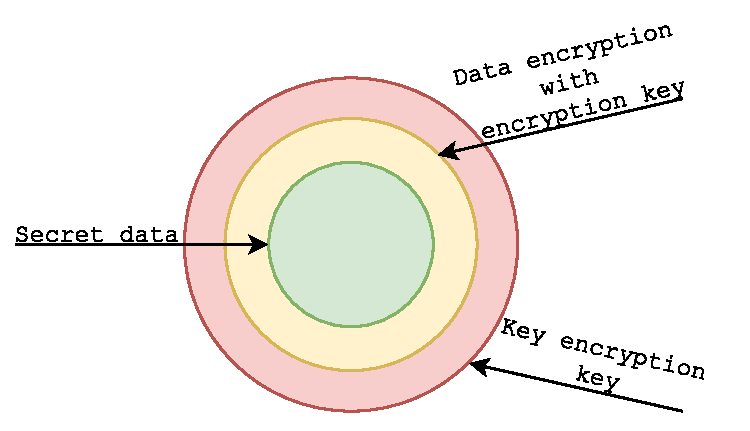
\includegraphics[scale=0.7]{figures/HowWeEncryptData.pdf}
    \caption{Hard drive encryption in a nutshell}
    \label{fig:encdata}
\end{figure}
Every encryption key should be unpredictable and unique set of bits able to "scramble" data in a way that it would be impossible to recover data whithout it.
To satisfy this need, encryption keys are generated by specialized algorithms such as AES (Advanced Encryption Standard\footnote{https://en.wikipedia.org/wiki/Symmetric-key\_algorithm\#Implementations}) for symmetric keys and RSA (Rivest–Shamir–Adleman\footnote{https://en.wikipedia.org/wiki/Public-key\_cryptography}) for asymmetric.
Changing encryption key implies the whole data decryption with old key and encryption with new encryption every time the old one is compromised or change is required.
Also this secret data might grow in size, and it is time and resource consuming to decrypt and encrypt the volume or even the whole hard drive.
Because of that the encryption key is then wrapped by the key encryption key.

Key encryption key is mostly generated using the user provided password.
This key encryption key is then used to encrypt encryption key which does the actual data encryption.
Again the most unsecure thing in this would be the user provided password which we can easily replace with using only cryptographically stronger key.
This principle has at least two advantages.
Changing the key encryption key does not affect encrypted data, and key can be changed whenever user desire to, and redistributed to all users or services who are supposed to access this data.

Hard drive could be encrypted as whole or per partition.
Full disk encryption is done in a way that all content on hard drive except MBR(Master Boot Record) is encrypted.
Encrypting MBR would make impossible to start boot sequence of the operating system.
Boot sequence would prompt user for key encryption key in order to load operating system from encrypted storage.

This could disrupt our daily basis and might be the reason why most of us do not use hard drive encryption, even when we know it will protect our data.
There is a way to automate hard drive unlocking on early boot with a help from key management system.
We can get the key encryption key from some remote system, the Escrow server mentioned in section \ref{escrow} Escrow server, or recover it with Tang described in chapter \ref{tang} Tang server.
Before that, let us have a look on most common hard drive encryption implementations.

\section{LUKS specification}\todo{master key hmm refactor text add example}

LUKS (Linux Unified Key Setup) is a platform-independent disk encryption specification.
It was created by Clemens Fruhwirth in 2004 and was originally intended for Linux distributions.

Referential implementation of LUKS, which was originally meant for Linux, is using a dm-crypt subsystem for bulk data encryption.
This subsystem is not particularly bound to LUKS.
Alongside Linux implementation exists LibreCrypt, the Windows implementation based on original FreeOTFE \cite{FreeOTFE} project by Sarah Dean.

A LUKS partition can have as many user passwords as there are available key slots, and to access the partition, the user has to provide only one of these passwords \cite{LUKS}.

Hard drive with a LUKS partition has notable structure, see Figure \ref{fig:luksvol}.
The entire partition start with the LUKS partition header containing the key material.
After header there is section with bulk data, which are encrypted with the master key.

\begin{figure}[h]
    \centering
    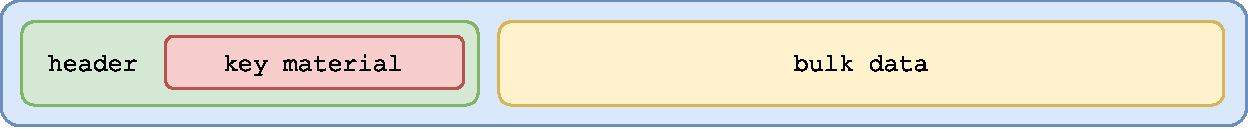
\includegraphics[scale=0.7]{figures/LUKSdrive.pdf}
    \caption{LUKS volume structure}
    \label{fig:luksvol}
\end{figure}

Header, also marked as {\it phdr}, contains information about the used cipher, cipher mode, the key length, a uuid and a master key checksum.
Also, the {\it phdr} contains information about the key slots.
Every key slot is associated with a key material section after the {\it phdr}.
When a key slot is active, the key slot stores an encrypted copy of the master key in its key material section.
This encrypted copy is locked by a user password.
Structure of key slot is on Figure \ref{fig:luksslot}.

\begin{figure}[h]
    \centering
    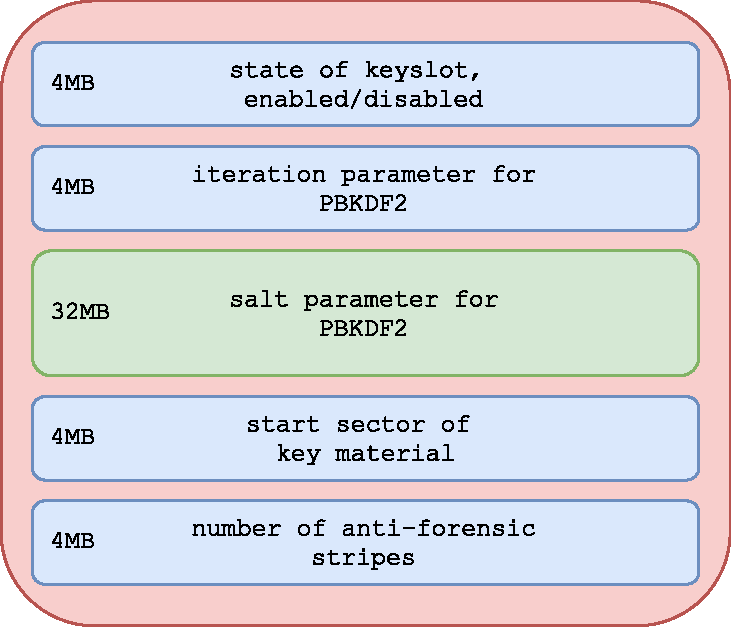
\includegraphics[scale=0.6]{figures/LUKSkeyslot.pdf}
    \caption{LUKS Key Slot}
    \label{fig:luksslot}
\end{figure}

\subsection{Encrypting with LUKS} \todo{ask for help with structure}

Creating a LUKS volume might be quite tough process.
Hard drive partition must contain the LUKS header just before the encrypted data.
Lets sum up the easier way first.

In case we have not installed our Linux operation system yet, we could simply select an option in time of installation.
Then the installation wizard will most likely asks for pass phrase - the key encryption key.
To demonstrate this, screen shots with Fedora 25 system installation can be found on appendix \ref{luksinstall}.

If we have already system installed with lots of data on partition, process will probably last longer and the procedure will be more complex.
There is no way you can encrypt whole system disk with LUKS without unmounting partition to encrypt.
For this purpose was developed {\it luksipc}, the LUKS In-Place Conversion Tool \cite{luksipc}.
Steps to encrypt disk using {\it luksipc} are on appendix \ref{luksipc}.

\section{Bit Locker} \todo{brief info}

BitLocker is a full disk encryption feature included with Windows Vista and later.
It is designed to protect data by providing encryption for entire volumes.
By default it uses the AES encryption algorithm in cipher block chaining (CBC) or XTS mode[6] with a 128-bit or 256-bit key.
[7][8] CBC is not used over the whole disk; it is applied to each individual sector.[9]
